\chapter {Analýza}

\section {Magnetická rezonancia}

Magnetická rezonancia (MR) je jedna zo zobrazovacích techník, ktorá je používaná k zobrazeniu vnútorných orgánov tela.
Narozdiel od röntgenového žiarenia a počítačovej tomografie (CT), magnetická rezonancia nepoužíva ionizujúce žiarenie. Avšak medzi spoločné znaky týchto troch zobrazovacích techník patrí ich neinvazívnosť a bezbolestné vyšetrenie \cite{basic_principles_of_mri} (vlastný preklad). \newline

Magnetická rezonancia sa používa najmä pri:
\begin {itemize}
\item {podozrení na anomálie mozgu a miechy, nádory a cysty,}
\item {poranení kĺbov a mäkkých tkanív,}
\item {podozrení na srdcové problémy,}
\item {rozličných ochoreniach pečene a iných brušných orgánov, atď. \cite{mr_usage} (vlastný preklad).}
\end {itemize}

Pred niektorými MR procedúrami sa pacientovi môže intravenózne podať kontrastná látka, ktorá zlepší kontrast a vzájomnú odlíšiteľnosť orgánov a mäkkých tkanív \cite{contrast_agents}.

Bohužiaľ, existujú aj určité kontraindikácie, pri ktorých použitie MR pre daného človeka nie je možné.
Jedným z kontraindikácií je implantovaný kardiostimulátor, v prípade že nie je kompatibilný s MR prístrojom. Všeobecne sa za kontraindikáciu považuje použitie akéhokoľvek magnetického materiálu v tele. Taktiež je MR vyšetrenie kontraindikované ženám v prvom trimestri tehotenstva \cite{mr_contraindications}.

\subsection {Princíp magnetickej rezonancie}

Princípom magnetickej rezonancie je smerové magnetické pole (moment - $\mathcal{B}_{0}$) spojené s pohybom voľných jadier vodíku v tele subjektu. Tieto jadrá majú charakteristický pohyb (spin) vytvárajúci malý magnetický moment s určitým smerom (ktorý je náhodný) a veľkosťou. Keď je subjekt umiestnený vo veľkom magnetickom poli (v tubuse MR prístroja), voľné vodíkové jadrá sa zarovnajú v smere $\mathcal{B}_{0}$ (smer $y$) a vytvoria magnetický moment $\mathcal{M}$ paralelne k $\mathcal{B}_{0}$. Vodíkové jadrá začnú náhle prechádzať okolo smeru magnetického poľa ako gyroskopy -- toto správanie sa nazýva Larmorova precesia \cite{basic_principles_of_mri} (vlastný preklad).

\begin {center}
        \centering
        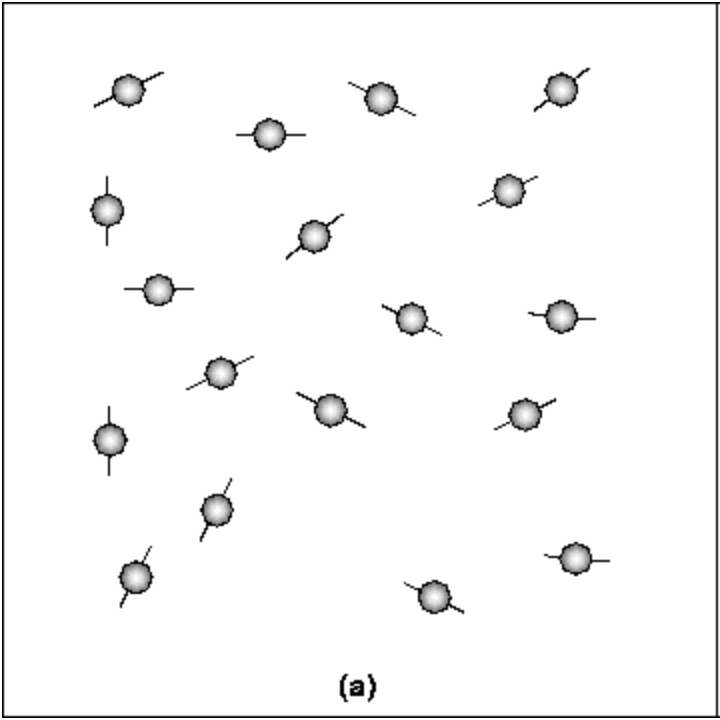
\includegraphics[width=6cm, height=6cm]{media/hydrogen/hydrogen_moving_freely.png}
        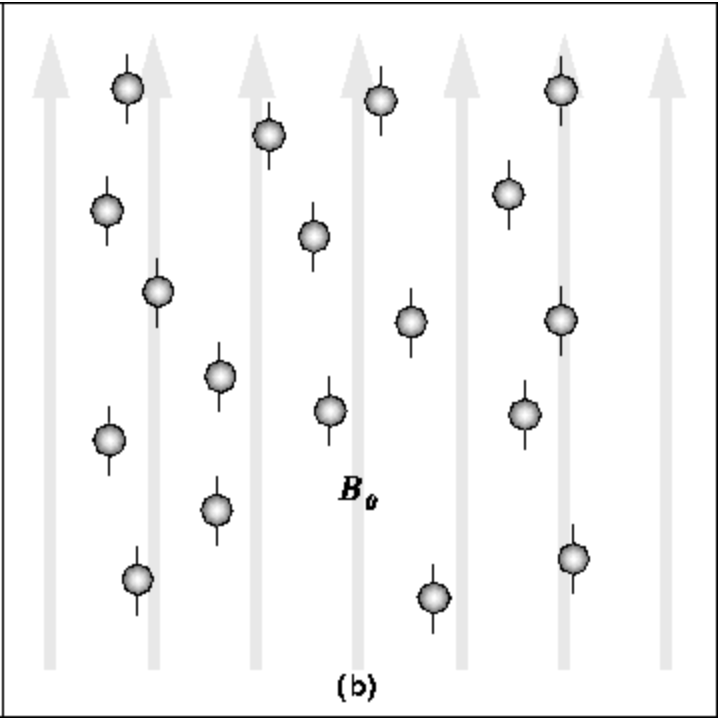
\includegraphics[width=6cm, height=6cm]{media/hydrogen/hydrogen_oscilating.png}
        \captionof{figure}[Voľný pohyb vodíkových jadier a ich zarovnanie v smere $\mathcal{B}_{0}$]{Na ľavom obrázku je možné vidieť voľný pohyb vodíkových jadier a na pravom ich zarovnanie v smere $\mathcal{B}_{0}$ \cite{basic_principles_of_mri}.}
\end {center}

Následne sa aplikuje rádiofrekvenčný impulz $\mathcal{B}_{rf}$ kolmo na $\mathcal{B}_{0}$.
Tento impulz rovnajúci sa frekvencii Larmorovej precesie spôsobí posun $\mathcal{M}$ od $\mathcal{B}_{0}$ \cite{basic_principles_of_mri} (vlastný preklad).

\begin {center}
        \centering
        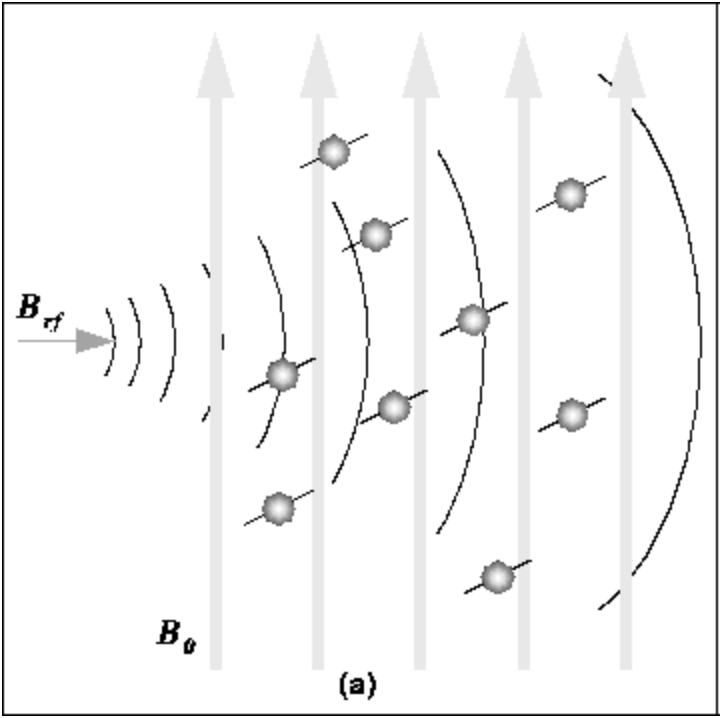
\includegraphics[width=6cm, height=6cm]{media/hydrogen/hydrogen_reacting_to_rf.png}
        \captionof{figure}[Kolmá aplikácia RF impulzu $\mathcal{B}_{rf}$ na vodíkové jadrá]{Kolmá aplikácia RF impulzu $\mathcal{B}_{rf}$ na vodíkové jadrá \cite{basic_principles_of_mri}.}
\end {center}

Frekvenciu Larmorovej precesie (nazývaná ako Larmorova frekvencia), je definovaná nasledovne:

\begin {center}
$\omega_{0}$ = $-\gamma * \mathcal{B}_{0}$,
\end {center}

kde $\gamma$ predstavuje gyromagnetický pomer a $\mathcal{B}_{0}$ intenzitu magnetického poľa.
Gyromagnetický pomer je konštanta závislá na jadre danej častice. Pre vodík sa táto konštanta rovná 42.6 MHz/Tesla \cite{basic_principles_of_mri} (vlastný preklad). \newline

Akonáhle prestane pôsobiť rádiofrekvenčný impulz $\mathcal{B}_{rf}$, jadrá vodíka sa presunú naspäť tak, že ich $\mathcal{M}$ je znovu paralelný s $\mathcal{B}_{0}$. Tento návrat vodíkových jadier sa nazýva relaxácia. Počas nej jadrá strácajú energiu vysielaním ich vlastného rádiofrekvenčného signálu. Tento signál sa nazýva \uv{voľný indukčný rozpad} -- z anglického Free Induction Decay (FID). Ten sa zmeria vodivým poľom MR prístroja za účelom vyhotovenia 3D MR snímku v odtieňoch šedej \cite{basic_principles_of_mri} (vlastný preklad).

\begin {center}
        \centering
        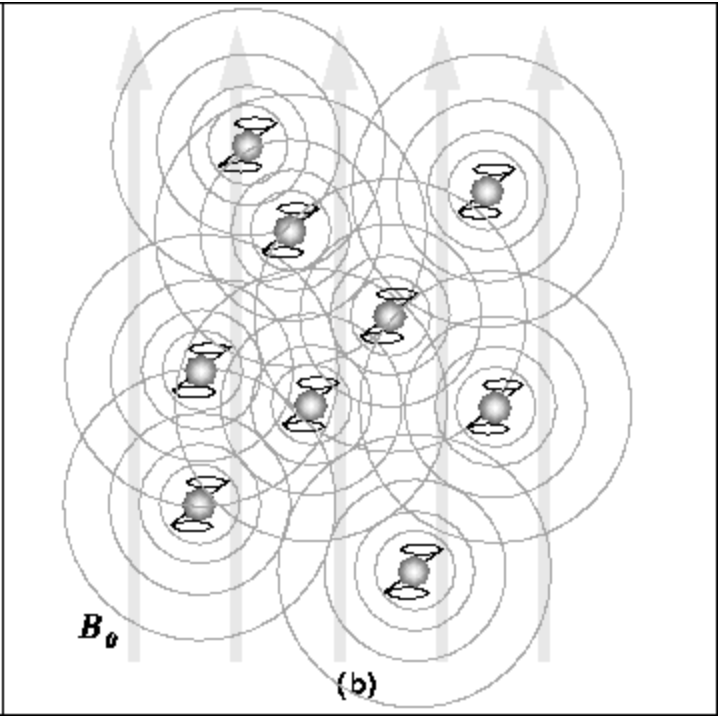
\includegraphics[width=6cm, height=6cm]{media/hydrogen/hydrogen_emitting_rf.png}
        \captionof{figure}[Emitovanie FID signálu vodíkovými jadrami]{Emitovanie FID signálu vodíkovými jadrami \cite{basic_principles_of_mri}.}
\end {center}

Avšak, na jeho vytvorenie musí byť FID signál enkódovaný pre každý rozmer pomocou frekvenčného a fázového kódovania. Kódovanie v axiálnom smere sa dosiahne pridaním gradientového magnetického poľa $\mathcal{G}_{y}$ v smere $\mathcal{B}_{0}$ (v smere $y$). Po pridaní $\mathcal{G}_{y}$ sa hodnota Larmorovej frekvencie zmení lineárne v axiálnom smere, tzn. že pre konkrétny axiálny rez existuje konkrétna Larmorova frekvencia, ktorá sa aplikuje vyslaním rádiofrekvenčného impulzu $\mathcal{B}_{rf}$. $\mathcal{G}_{y}$ sa potom odstráni a ďalší gradient, $\mathcal{G}_{x}$, sa aplikuje kolmo na $\mathcal{G}_{y}$. Výsledkom je, že rezonančné frekvencie jadier sa menia v smere $x$ vďaka $\mathcal{G}_{x}$ a majú fázovú variáciu v smere $y$ v dôsledku predtým aplikovaného $\mathcal{G}_{y}$. Vzorky v smere $x$ sú teda kódované frekvenciou a v smere $y$ fázou. 2D inverzná Fourierova transformácia sa následne použije pre transformáciu vzoriek na snímku \cite{basic_principles_of_mri} (vlastný preklad). \newline

Kontrast získanej snímky závisí od nasledujúcich dvoch parametrov:

\begin {itemize}
\item {od času pozdĺžnej relaxácie - T1}
\item {a od času priečnej relaxácie - T2.}
\end {itemize}

Čas T1 je čas potrebný pre jadrá vodíkov k ich relaxácii a čas T2 predstavuje čas za ktorý sa FID signál prechádzajúci cez dané tkanivo rozpadne. Oba časy závisia od daného typu látky nachádzajúcej sa v subjekte \cite{basic_principles_of_mri} (vlastný preklad).

Po získaní MR snímky sa impulz $\mathcal{B}_{rf}$ opakuje vopred stanovenou rýchlosťou. Zmenou sekvencie impulzov ($\mathcal{B}_{rf}$) sa vytvárajú rôzne typy snímkov. Čas opakovania ($TR$) je množstvo času medzi po sebe nasledujúcimi pulznými sekvenciami aplikovanými na rovnaký rez. Time to Echo ($TE$) je čas medzi dodaním impulzu $\mathcal{B}_{rf}$ a prijatím odozvy. Úpravou $TR$ je možné meniť výsledný kontrast na snímke medzi rôznymi typmi tkanív \cite{basic_principles_of_mri} (vlastný preklad). \clearpage

\section {SPAMM}

SPAMM -- z anglického (SPAtial Modulation of Magnetization) $\rightarrow$ \uv{priestorová modulácia magnetizácie} -- je technika používajúca rádiofrekvenčné saturačné impulzy pre umiestnenie mriežky na myokard, za cieľom sledovania jeho pohybu počas srdcového cyklu.

V súčasnej praxi sa SPAMM technika používa v situáciách, kde informácia o kontrakcii myokardu je kľúčová, ako napr. podozrenie na ischemickú chorobu srdca alebo abnormality týkajúcej sa neprirodzeného pohybu steny myokardu \cite{spamm_description} (vlastný preklad).

\begin {center}
        \centering
        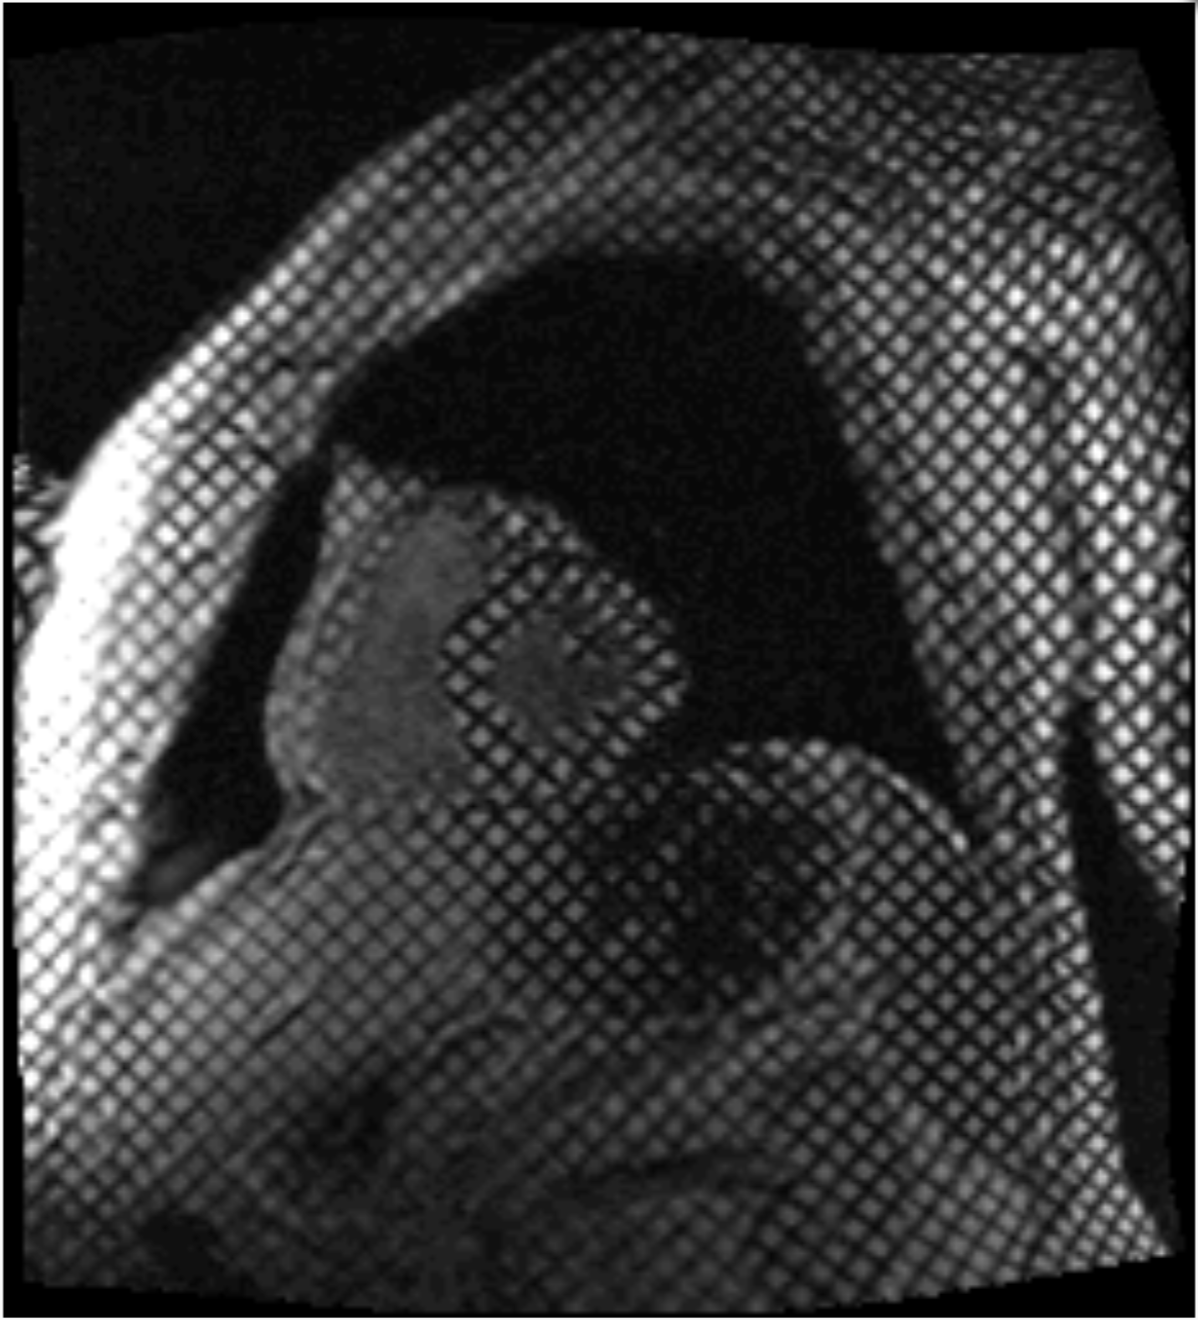
\includegraphics[width=6cm, height=6cm]{media/heart/tagged_heart.png}
        \captionof{figure}[Tagovaný snímok myokardu pomocou techniky SPAMM]{Otagovaný snímok myokardu pomocou techniky SPAMM \cite{spamm_description}.}
\end {center}

Nevýhodou použitia tejto techniky je skutočnosť, že táto mriežka sa stráca s blížiacim sa koncom srdcového cyklu. Samotné čiary mriežky sa pri konci systoly (časť srdcového cyklu, počas ktorej sa komory srdca sťahujú po naplnení krvou) môžu zlúčiť alebo úplne vyblednúť, čo sťažuje následnú analýzu pohybu srdca \cite{spamm_description} (vlastný preklad).

\begin {center}
        \centering
        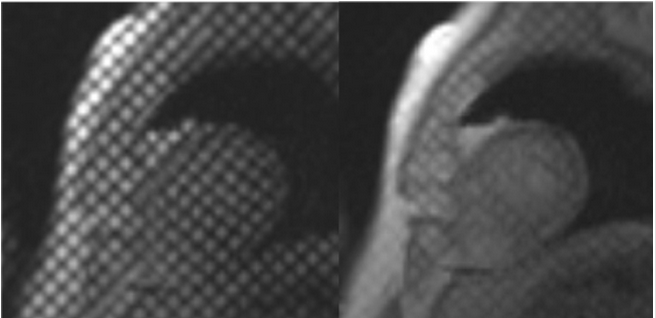
\includegraphics[width=10cm, height=5cm]{media/heart/early_late_systole.png}
        \captionof{figure}[Ukážka vyblednutia SPAMM mriežky]{Ľavý obrázok zobrazuje začiatok systoly, pravý jej koniec.}
\end {center}

\section {Analýza súčasnej aplikácie}

Táto sekcia sa zaoberá účelom súčasnej aplikácie a analýzou použitých technológií, ktoré sú dôležité pre celkovú funkcionalitu aplikácie. Následne sú popísané podprogramy, ktoré riešia výpočtovo náročnejšie úlohy v rámci tejto aplikácie. Jednému z najdôležitejších podprogramov, \texttt{grid-tracker}, je venovaná väčšia pozornosť. Táto sekcia sa taktiež venuje následnému zostaveniu a spusteniu aplikácie, ktoré je dôležité pre následnú analýzu používateľského rozhrania aplikácie.

\subsection {Účel aplikácie}

Účelom súčasnej aplikácie -- DICOM Viewer -- je analýza pohybu srdcového svalu, pomocou ktorej by bolo možné zistiť anomálie v jeho pohybe. Aplikácia umožňuje importovať súbory typu DICOM (popísaného v sekcii \ref{dicom}), ktoré sú otagované SPAMM mriežkou. Na importovaných snímkach je následne používateľom vytvorená mriežka. Štruktúra a parametre týchto mriežok sú potom poslané podprogramu \texttt{grid-tracker}, ktorého úlohou je zarovnanie používateľom vytvorených mriežok s mriežkami vytvorenými SPAMM technikou. Po ich zarovnaní mriežky je možné pomocou techniky grafových rezov odsegmentovať srdečné komory a tým pádom zúžiť analýzu pohybu srdcového svalu len na tieto komory.

Táto diplomová práca sa zameriava na vytvorenie webovej verzie súčasnej aplikácie vrátane zarovnania mriežok pomocou \texttt{grid-tracker} podprogramu \ref{helper_apps}.

\subsection {Použité technológie}

Popisu použitých technológií v súčasnej desktopovej aplikácii sa venuje táto podsekcia. Na základe zistenia, aké technológie a aplikačné závislosti aplikácia využíva, bude nakoniec možné aplikáciu zostaviť a vyskúšať. Nasledujúci prehľad použitých technológií je založený na dôslednom preštudovaní zdrojového kódu aplikácie, ktorý sa vyznačoval skoro neexistujúcou dokumentáciou. Bez tejto dokumentácie bola orientácia v zdrojovom kóde sťažená a tým pádom sa čas potrebný pre analýzu celkovej architektúry aplikácie značne predĺžil.

\subsubsection {Qt}

\quad Súčasná aplikácia bola vyvinutá pomocou Qt -- cross-platformového frameworku určeného pre vytváranie aplikácií najmä v jazyku C\texttt{++}. Aplikácie vyvinuté týmto frameworkom majú výhodu v tom, že sú spustiteľné na rôznych operačných systémoch s minimálnym počtom zmien v zdrojovom kóde \cite{qt_description} (vlastný preklad). V súčasnosti (od roku 2014) zastrešuje vývoj tohto frameworku spoločnosť The Qt Company.

Výsadou Qt frameworku je taktiež rozdelenie jeho funkcionality do jednotlivých modulov. Pri následom vytváraní aplikácie sa použijú len také moduly, ktoré sú v danej aplikácii potrebné \cite{qt_description} (vlastný preklad).

Existujúca aplikácia využíva tento framework vo verzii 5.15, ktorá sa vyznačuje tým, že je to verzia s dlhodobou podporou. Koniec podpory tejto verzie je naplánovaný na 26.5.2023. Najnovšia verzia Qt frameworku je momentálne verzia 6.4 a čo sa týka najnovšej verzie s dlhodobou podporou, tou je Qt vo verzii 6.2.

V súčasnej desktopovej aplikácii boli použité nasledovné moduly: 

\begin{itemize}
\item {Qt Core}
\item {Qt Widgets}
\item {Qt GUI}
\item {Qt Test}
\end{itemize}

Qt Core modul obsahuje najpoužívanejšie triedy ako napr. \texttt{QCoreApplication}, \texttt{QObject}, \texttt{QDebug} a iné. Nakoľko sú tieto triedy používané aj inými modulmi, je tento modul implicitne nalinkovaný Qt frameworkom pri budovaní aplikácie \cite{qtcore_description} (vlastný preklad). \newline

Qt Widgets modul poskytuje UI elementy, ktoré sú určené pre vytváranie používateľského rozhrania. Tieto elementy môžu zobrazovať rozličné dáta, prijímať vstup z klávesnice, byť štylizované a zoskupované do rozličných usporiadaní \cite{qtwidgets_description} (vlastný preklad). Existujúca aplikácia používa z modulu napr. triedu \texttt{QMainWindow}, ktorá je zodpovedná za vykreslenie aplikačného okna a taktiež triedu \texttt{QGraphicsScene}, ktorá je zodpovedná za vykreslenie snímkov z magnetickej rezonancie v DICOM formáte. \newline

Qt GUI modul obsahuje triedy určené pre zobrazovanie aplikačného okna a iného grafického obsahu s následnou obsluhou udalostí. Taktiež obsahuje triedy, ktoré sú zodpovedné za zobrazovanie 2D grafiky, fontov a typografie \cite{qtgui_description} (vlastný preklad).
Súčasná aplikácia z tohto modulu používa napr. triedu \texttt{QImage}, ktorá obsahuje metódy pre priamy prístup k pixelom snímkov a ich manipuláciu. \newline

Qt Test modul poskytuje rozličné triedy pre jednotkové testovanie Qt aplikácií a príslušných knižníc \cite{qttest_description} (vlastný preklad) -- v súčasnej aplikácii bol tento modul využitý pri testovaní grafického používateľského rozhrania a funkcionalít súčasnej aplikácie, ako napr. testovanie zmien v nastaveniach vykreslenej mriežky na obrázku z magnetickej rezonancie.

\subsubsection {Qmake}\label{qmake}

Pre zjednodušenie písania Makefilov, ktoré definujú, ako má byť program skompilovaný, bol použitý nástroj Qmake. Tento nástroj pochádza taktiež z dielne The Qt Company. Qmake umožňuje vývojárom definovať vytváranie rozličných Makefilov pre daný program pomocou syntaxu definovaného programom Qmake \cite{qmake_description} (vlastný preklad). Výsledkom tohto procesu je súbor s príponou \texttt{.pro} obsahujúci inštrukcie, ako daný Makefile vytvoriť. Následne sa pomocou príkazu \texttt{qmake} s argumentom cesty k \texttt{.pro} súboru vytvorí \texttt{Makefile} súbor, pomocou ktorého je možné daný program skompilovať, čoho výsledkom je spustiteľný súbor aplikácie.

Pre súčasnú aplikáciu sa daný súbor volá \texttt{Cameo.pro} a nachádza sa v adresári \texttt{dicomViewer}.

\subsubsection {DICOM}\label{dicom}

V súčasnosti sú snímky získané pomocou zobrazovacích techník v medicíne zväčša ukladané v archivačnom a komunikačnom systéme snímkov. Tento systém ukladá nielen snímkové dáta ale aj iné relevantné dáta k týmto snímkam podľa štandardu známom ako DICOM (Digital Imaging and Communications in Medicine) \cite{Varma_2012} (vlastný preklad). Ten je medzinárodným štandardom pre komunikáciu a manažment informácií o medicínskych obrazových a k nim príslušných dátach. Definuje, ako majú byť takéto dáta spracovávané, ukladané, tlačené a prenášané medzi zariadeniami podporujúcimi príjem týchto dát \cite{about_dicomlibrary} (vlastný preklad).

Začiatok vývoja DICOM štandardu sa datuje k prelomu 80. a 90. rokoch 20. storočia, kedy započala spolupráca medzi American College of Radiology a National Electrical Manufacturers Association (NEMA). NEMA taktiež vlastní autorské práva k tomuto štandadu. Momentálne sa DICOM skladá z 22 nezávislých častí, z ktorých avšak nie všetky musia byť implementované daným zariadením podporujúcim tento štandard \cite{dicom_history} (vlastný preklad).

Pre účely spracovania snímkových dát, DICOM štandard vo svojej 10. časti definuje dátovú štruktúru (formát) súboru, do ktorého sa tieto dáta ukladajú. Dátová štruktúra súboru, ktorý spĺňa podmienky 10. časti tohto štandaru, býva značená ako \uv{DICOM Part 10} súbor, inak známy ako DICOM súbor \cite{Varma_2012} (vlastný preklad).

Štruktúra tohto (binárneho) súboru je nasledovná -- prvých 128 bajtov býva zväčša prázdnych (vyplnených 0). Ďalšie 4 bajty obsahujú uložený reťazec \uv{DICM}.  Na základe týchto bajtov sa dá určiť, či sa jedná alebo nejedná o DICOM súbor.
Ďalej nasleduje hlavička, ktorá je rozdelená na viacero skupín zoskupujúcich súvisiace atribúty. Konkrétne atribúty sa adresujú tagom - ten sa skladá z 8 čísiel v hexadecimálnom formáte. Prvé 4 čísla reprezentujú skupinu, v ktorej sa daný atribút nachádza a posledné 4 čísla jednoznačne identifikujú konkrétny atribút v skupine \cite{Varma_2012} (vlastný preklad).

Ako príklad bude uvedené získanie informácie o pacientovom veku - všetky informácie o pacientovi sa nachádzajú v skupine 0010. Pacientov vek v tejto skupine sa nachádza na pozícii 1010, tým pádom výsledný tag pod ktorým nájdeme vek pacienta je (0010, 1010). Ku každému tagu je jednoznačne priradená reprezentácia jej hodnoty (VR), ktorý určuje dátový typ, formát a dĺžku hodnoty daného atribútu  \cite{Varma_2012} (vlastný preklad).

Po hlavičke nasleduje skupina 7FE0, ktorá už obsahuje dáta o samotných obrazových pixeloch \cite{Varma_2012} (vlastný preklad). Typ kódovania týchto dát určuje Transfer Syntax -- ten udáva, akým spôsobom sú obrazové pixely zakódované. Transfer Syntax obsahuje taktiež informáciu, v akom poradí bajtov sú informácie zakódované (Little Endian vs Big Endian) a aká kompresia obrazových dát bola použitá \cite{dicom_transfer_syntax} (vlastný preklad).

\subsubsection {DCMTK}\label{dcmtk}

DCMTK je knižnica, ktorá implementujú veľkú časť DICOM štandardu v jazykoch C a C\texttt{++}. Úlohou tejto knižnice je okrem iného skúmanie, vytváranie a konverzia DICOM súborov, manipulácia s pamäťovými médiami a odosielanie, resp. prijímanie obrazových súborov cez internetové pripojenie. Za jej vývojom stojí nemecká firma OFFIS, ktorá túto knižnicu vyvíja nepretržite už od roku 1993. V súčasnosti sa používa v nemocniciach a rôznych spoločnostiach po celom svete, kde predstavuje softvérový základ pri rozličných výskumných projektoch, prototypoch a komerčných produktoch nevynímajúc \cite{dcmtk_description} (vlastný preklad). \newline

Súčasná aplikácia je kompatibilná s najnovšou verziou tejto knižnice, ktorou je verzia 3.6.7. DCMTK knižnica je v tejto aplikácii použitá pre získanie informácií z hlavičiek DICOM súborov, ako napr:

\begin{itemize}
\item {údaje o pacientovi,}
\item {údaje o snímku a}
\item {údaje o sérií snímkov.}
\end{itemize}

\subsubsection {OpenMP}

OpenMP poskytuje rozhranie pre programovanie aplikácií (tzv. API), vďaka ktorému je možné vytvárať C, C\texttt{++} a Fortran aplikácie využívajúce viac vlákien nad zdieľanou pamäťou. Vývoj OpenMP v súčasnosti zastrešuje OpenMP Architecture Review Board.
OpenMP funguje na báze direktív, pomocou ktorých sa jednotlivé časti programu dajú paralelizovať viacerými spôsobmi -- a to paralelizáciou prevádzania jednotlivých úloh (tzv. funkčný paralelizmus -- vhodný pre paralelizáciu rekurzívnych algoritmov, kde úloha = volanie funkcie) alebo paralelizáciou dátovo nezávislých for loop iterácií (tu sa jedná o tzv. iteračný dátový paralelizmus) \cite{openmp_description}.

Existujúca aplikácia využíva direktívy OpenMP pre paralelizáciu výpočetne náročnejších algoritmov. Súčasná verzia OpenMP, verzia 5.2, je plne kompatibilná s aktuálnym zdrojovým kódom aplikácie.

\subsubsection {TNL}\label{tnl}

Template Numerical Library, v skratke TNL, je numerická knižnica, ktorá poskytuje rozličné dátové štruktúry, ktoré uľahčujú prácu s pamäťou a vývoj efektívnych numerických riešičov. Táto knižnica je implementovaná pomocou C\texttt{++} s cieľom poskytnúť flexibilné a užívateľsky prívetivé rozhranie. TNL poskytuje natívnu podporu pre moderné hardwarové architektúry ako sú viacjadrové CPU, GPU a distribuované systémy, ktoré je možné spravovať cez jednotné rozhranie \cite{tnl_description}.

Vývoj TNL knižnice od jej počiatku riadi Tomáš Oberhuber z Katedry matematiky na FJFI ČVUT v spolupráci s Jakubom Klinkovským a Alešom Wodeckim.

V súčasnej aplikácii sú z TNL knižnice použité kolekcie ako napr. \texttt{String} pre manipuláciu s reťazcami a \texttt{Containers::Array}, \texttt{Containers::\{Vector,StaticVector,MultiVector\}}, čo sú šablóny pre reprezentáciu n-dimenzionálnych polí, ktoré abstrahujú manažment dát a exekúciu bežných operácií na rozličných hardvérových architektúrach.

Aplikácia z TNL knižnice taktiež používa \texttt{Solvers::ODE::Merson} -- jedná sa o Runge-Kutta-Merson metódu štvrtého rádu s adaptívnym výberom časového kroku, pomocou ktorej vieme získať približné riešenie diferenciálnych rovníc.

Bohužiaľ, súčasná aplikácia nie je kompatibilná s najnovšími zdrojovými kódmi TNL knižnice -- pre nájdenie posledného \uv{dobrého stavu} knižnice, t.j. stavu za ktorého bolo možné aplikáciu skompilovať, bol využitý nástroj \texttt{git bisect}. Tento nástroj našiel ako posledný \uv{dobrý stav} knižnice z 13.5.2021. Pri využití TNL knižnice zostavenej po tomto dátume nebolo možné súčasnú aplikáciu skompilovať.

\subsection {Pomocné podprogramy}\label{helper_apps}

Súčasná aplikácia obsahuje a využíva nasledujúce 3 podprogramy:

\begin {itemize}
\item {grid-tracker}
\item {local-variance}
\item {graph-cuts}
\end {itemize}

\texttt{grid-tracker} podprogram je určený pre sledovanie pohybu myokardu pomocou detekcie SPAMM mriežky z DICOM snímku a mriežky vytvorenej používateľom. Mriežku vytvorenú používateľom sa snaží zarovnať so SPAMM mriežkou pre každú snímku zo sekvencie snímkov. Výstupom sú upravené koordináty bodov mriežky vytvorenej používateľom -- tie sa následne aplikujú namiesto doterajšej mriežky, čoho výsledkom je zobrazenie mriežky s upravenými koordinátmi bodov. \newline

Vstupom tohto programu sú nasledujúce parametre:
\begin {itemize}
\item {\texttt{inputImageFileNames} -- vektor reťazcov reprezentujúce cesty k súborom multivektorov (definované TNL knižnicou), ktoré obsahujú enkódované DICOM snímky,}
\item {\texttt{inputGridFileNames} -- vektor reťazcov reprezentujúce cesty k súborom používateľom definovaných mriežok uložených ako TNL textový multivektor,}
\item {\texttt{outputGridFileNames} (nepovinné)-- vektor reťazcov reprezentujúce cesty k súborom spracovaných mriežok, ktoré budú uložené ako textový TNL multivektor,}
\item {\texttt{curvatureCoefficient} -- závislosť vývoja mriežky od zakrivenia, vyššie číslo znamená vyššiu závislosť,}
\item {\texttt{forceCoefficient} -- závislosť mriežky od gradientu obrazu, vyššie číslo znamená vyššiu závislosť,}
\item {a \texttt{stopTime} -- časový interval algoritmického výpočtu.}
\end {itemize}

Jeho výstupom sú predchádzajúce používateľom definované mriežky v textovom TNL multivectore upravené algoritmom tak, aby mriežky zodpovedali mriežkam definovanými SPAMM metódou. \newline

Nasledujúce dva podprogramy nie sú dôležité pre túto diplomovú prácu, avšak pre úplnosť je ich účel vysvetlený. \newline

Úlohou \texttt{local-variance} podprogramu je aplikovanie filtra lokálnej variancie pre danú snímku za účelom neskoršej lepšej segmentácie srdcových komôr. Tento filter je implentovaný pomocou jednoduchého rozptylového filtru, ktorý vypočíta priemernú intenzitu pixelov vo štvorcovom okolí každého pixelu a túto hodnotu dosadí do výberového rozptylu, ktorý sa bude rovnať novej hodnote intenzity pixelu \cite{master_thesis_app}.

Podprogram \texttt{graph-cuts} slúži pre segmentáciu srdcových komôr, ktorá vychádza z predpokladu, že hranica medzi objektom a jeho pozadím sa nachádza v miestach nekonzistencie susedných pixelov snímky. Implementovaná metóda, ktorá dosiahla dobré výsledky bola metóda grafových rezov, kombinujúca Fordov-Fulkersonovým algoritmom s Preflow-Push algoritmom \cite{master_thesis_app}.

\subsection {Zostavenie aplikácie a jej spustenie}

Pre potrebu popísania používateľského rozhrania je najprv žiaduce dosiahnuť zostavenie existujúcej aplikácie a jej následné spustenie. Po počiatočnej analýze zdrojového kódu, v ktorom bolo zistené, že aplikácia bola vyvíjaná pre Linuxové prostredie, bol vo virtuálnom prostredí nainštalovaný operačný systém Ubuntu 22.10.

Pre zostavenie súčasnej aplikácie bude potrebné nainštalovať Qt framework spolu s nástrojom Qmake, nakoľko ich architektúra súčasnej aplikácia vyžaduje.

Pre inštaláciu Qmake nástroja je potrebné nainštalovať balíček \texttt{qt5-default}. Ten obsahuje nie len nástroj \texttt{qmake} ale aj aplikáciu Qt Creator.

Qt Creator je aplikácia, ktorá poskytuje prostredie pre integrovaný vývoj aplikácií postavených nad Qt frameworkom. Pomocou tejto aplikácie je možné vyvíjať, testovať, zostavovať, spúšťať a debugovať aplikácie postavené na tomto frameworku. Táto aplikácia bude neskôr využitá pre neskorší debugging súčasnej aplikácie.

Okrem balíčku \texttt{qt5-default} je taktiež potrebné nainštalovať balíčky \texttt{cmake} a \texttt{build-essential}, čo sú balíčky poskytujúce ďalšie nástroje potrebné pre úspešné zostavenie aplikácie. Tieto balíčky v niektorých prípadoch už môžu byť súčasťou použitej linuxovej distribúcie, čo ale neplatilo v prípade použitia Ubuntu 22.10 ako operačného systému.

Pretože súčasná aplikácia využíva DCMTK knižnicu, ako bolo popísané v sekcii \ref{dcmtk}, je tiež nutné nainštalovať nasledujúce balíčky: \texttt{dcmtk} a {\texttt{libdcmtk-dev}.

Prvý z uvedených balíčkov nainštaluje samotnú DCMTK knižnicu, druhý obsahuje knižnice a hlavičkové súbory pre vývoj aplikácií používajúce túto knižnicu. Nakoľko v \texttt{Dicom.pro} súbore (ktorý je určený pre výsledné zostavenie aplikácie) sa nachádzajú cesty ku knižniciam z balíčku \texttt{libdcmtk-dev}, je aj tento balíček nutný nainštalovať pre neskoršie korektné spustenie súčasnej aplikácie.

Keďže \texttt{grid-tracker} podprogram obsahuje OpenMP direktívy pre paralelizáciu výpočetných algoritmov, je potrebné nainštalovať OpenMP prostredníctvom balíčku \texttt{libomp-dev}. TNL knižnica bude taktiež benefitovať z inštalácie tohto balíčka, nakoľko sama využíva OpenMP pre paralelizáciu algoritmov, čo znamená, že sa tento balíček nainštaluje ešte pred samotnou inštaláciou TNL knižnice.

Ďalej je potrebné nainštalovať samotnú TNL knižnicu -- pre jej inštaláciu bude potrebné stiahnuť zdrojové kódy buď formou zabaleného zdrojového kódu v .zip balíčku, alebo naklonovaním repozitára pomocou programu \texttt{git}. Keďže aplikácia je nekompatibilná s najnovšou verziou TNL knižnice, je potrebné stiahnuť alebo naklonovať repozitár so zdrojovými kódmi do dátumu 13.5.2021 (viď \ref{tnl}).

Nakoľko je nutné samotnú knižnicu zo zdrojových kódov zostaviť, je nevyhnutné mať nainštalovaný kompilátor podporovaný samotnou knižnicou. Medzi podporované kompilátory sa radí GCC kompilátor vo verzii 8.0 a vyššie alebo Clang vo verzii 7.0 a vyššie. Prvý z nich je možné nainštalovať pomocou balíčku \texttt{gcc} a druhý pomocou balíčku \texttt{clang}.

Následne je potrebné exekuovať inštalačný skript \texttt{install}, ktorého účelom je nakonfigurovanie TNL knižnice a jej zostavenia.
Pred exekuovaním samotného inštalačného skriptu \texttt{install} je potrebné zistiť, či sú nainštalované balíčky \texttt{doxygen}, \texttt{matplotlib} a \texttt{graphviz}. Tieto balíčky sa využívajú pri generovaní dokumentácie počas exekúcie \texttt{install} skriptu (pri defaultnej inštalácii). Ak sa niektorý z daných balíčkov nenachádza v systéme, je potrebné ho doinštalovať.

Po nainštalovaní všetkých potrebných balíčkov nastal čas pre zostavenie TNL knižnice spustením \texttt{install} skriptu. Po jeho ukončení sa hlavičkové súbory TNL knižnice budú nachádzať v priečinku \texttt{/usr/lib/aarch64-linux-gnu}. Názov posledného priečinku sa môže líšiť, nakoľko je závislý na architektúre CPU, na ktorom sa TNL knižnice zostavuje. V tomto prípade bola knižnica zostavovaná na systéme Ubuntu 22.10 bežiacom nad CPU s architektúrou Aarch64 (Apple M1 Pro CPU).

Ďalším krokom pre úspešné zostavenie aplikácie je definovanie cesty k hlavičkovým súborom TNL knižnice v samotnom \texttt{Cameo.pro} súbore, určenom pre zostavenie aplikácie pomocou programu \texttt{qmake}. Po otvorení súboru \texttt{Cameo.pro} je teda potrebné nastaviť hodnotu premennej \lstinline{DCMTK_LIBS} -- v tomto prípade ju bolo potrebné nastaviť na \texttt{/usr/lib/aarch64-linux-gnu} a následne daný súbor uložiť.

Po prevedení všetkých predchádzajúcich krokoch je možné spustiť nástroj \texttt{qmake} pomocou krokov popísaných v sekcii \ref{qmake}. Jeho výsledkom bude \texttt{Makefile} súbor, ktorý definuje kroky, ako zostaviť súčasnú aplikáciu. V tomto momente je už možné súčasnú aplikáciu skompilovať pomocou spustenia príkazu \texttt{make install}.

Po skompilovaní aplikácie sa v rovnakom priečinku objaví spustiteľný súbor \texttt{Cameo}, ktorému je potrebné nastaviť práva pre spustenie príkazom \texttt{chmod +x Cameo}. Následne je možné spustiť aplikáciu príkazom \texttt{./Cameo}.

\subsection {Používateľské rozhranie}\label{old_ui}

Po úspešnom spustení aplikácie sa používateľovi zobrazí hlavné okno aplikácie.
V aplikačnom okne sa taktiež zobrazí menu s nasledovnými možnosťami:

\begin {enumerate}
\item {File}
	\begin {enumerate}
		\item {Open -- otvorí systémové okno pre výber priečinku s DICOM snímkami, ktoré sa majú importovať do aplikácie}
		\item {Save Image}
		\begin {enumerate}
			\item {Save View -- uloží pohľad na aktuálnu snímku vo zvolenom formáte}
			\item {Save Scene -- uloží scénu vo zvolenom formáte}
			\item {Save Area of Interes [sic] -- uloží plochu záujmu vo zvolenom formáte}
		\end {enumerate}
	\item {Save all selected}
		\begin {enumerate}
			\item {Save View -- uloží pohľad vybraných snímky vo zvolenom formáte}
			\item {Save Scene -- uloží scénu vybraných snímkov vo zvolenom formáte}
			\item {Save Area of Interes [sic] -- uloží plochu záujmu vybraných snímkov vo zvolenom formáte}
		\end {enumerate}	
	\item {Exit -- ukončí aplikáciu}
	\end {enumerate}
\item {Aditional [sic] Tools}
	\begin {enumerate}
	\item {Grid Tools -- otvorí ľavý postranný panel aplikácie s nastavením mriežky}
	\item {Lvf Tools -- otvorí ľavý postranný panel aplikácie s nastavením filtru lokálnej variácie}
	\item {Graph Cuts Tools -- otvorí ľavý postranný panel aplikácie s nastavením grafových rezov}
	\end {enumerate}
\item {Help}
	\begin {enumerate}
	\item {About -- zobrazí informácie o DICOM Viewer aplikácii}
	\end {enumerate}
\end {enumerate}

Po spustení sa aplikácia nachádza v stave, v ktorom nie je možné s ňou interagovať -- inými slovami, je najprv potrebné do aplikácie importovať snímky v DICOM formáte, ako je ukázané na obrázku nižšie.

\begin {center}
        \centering
        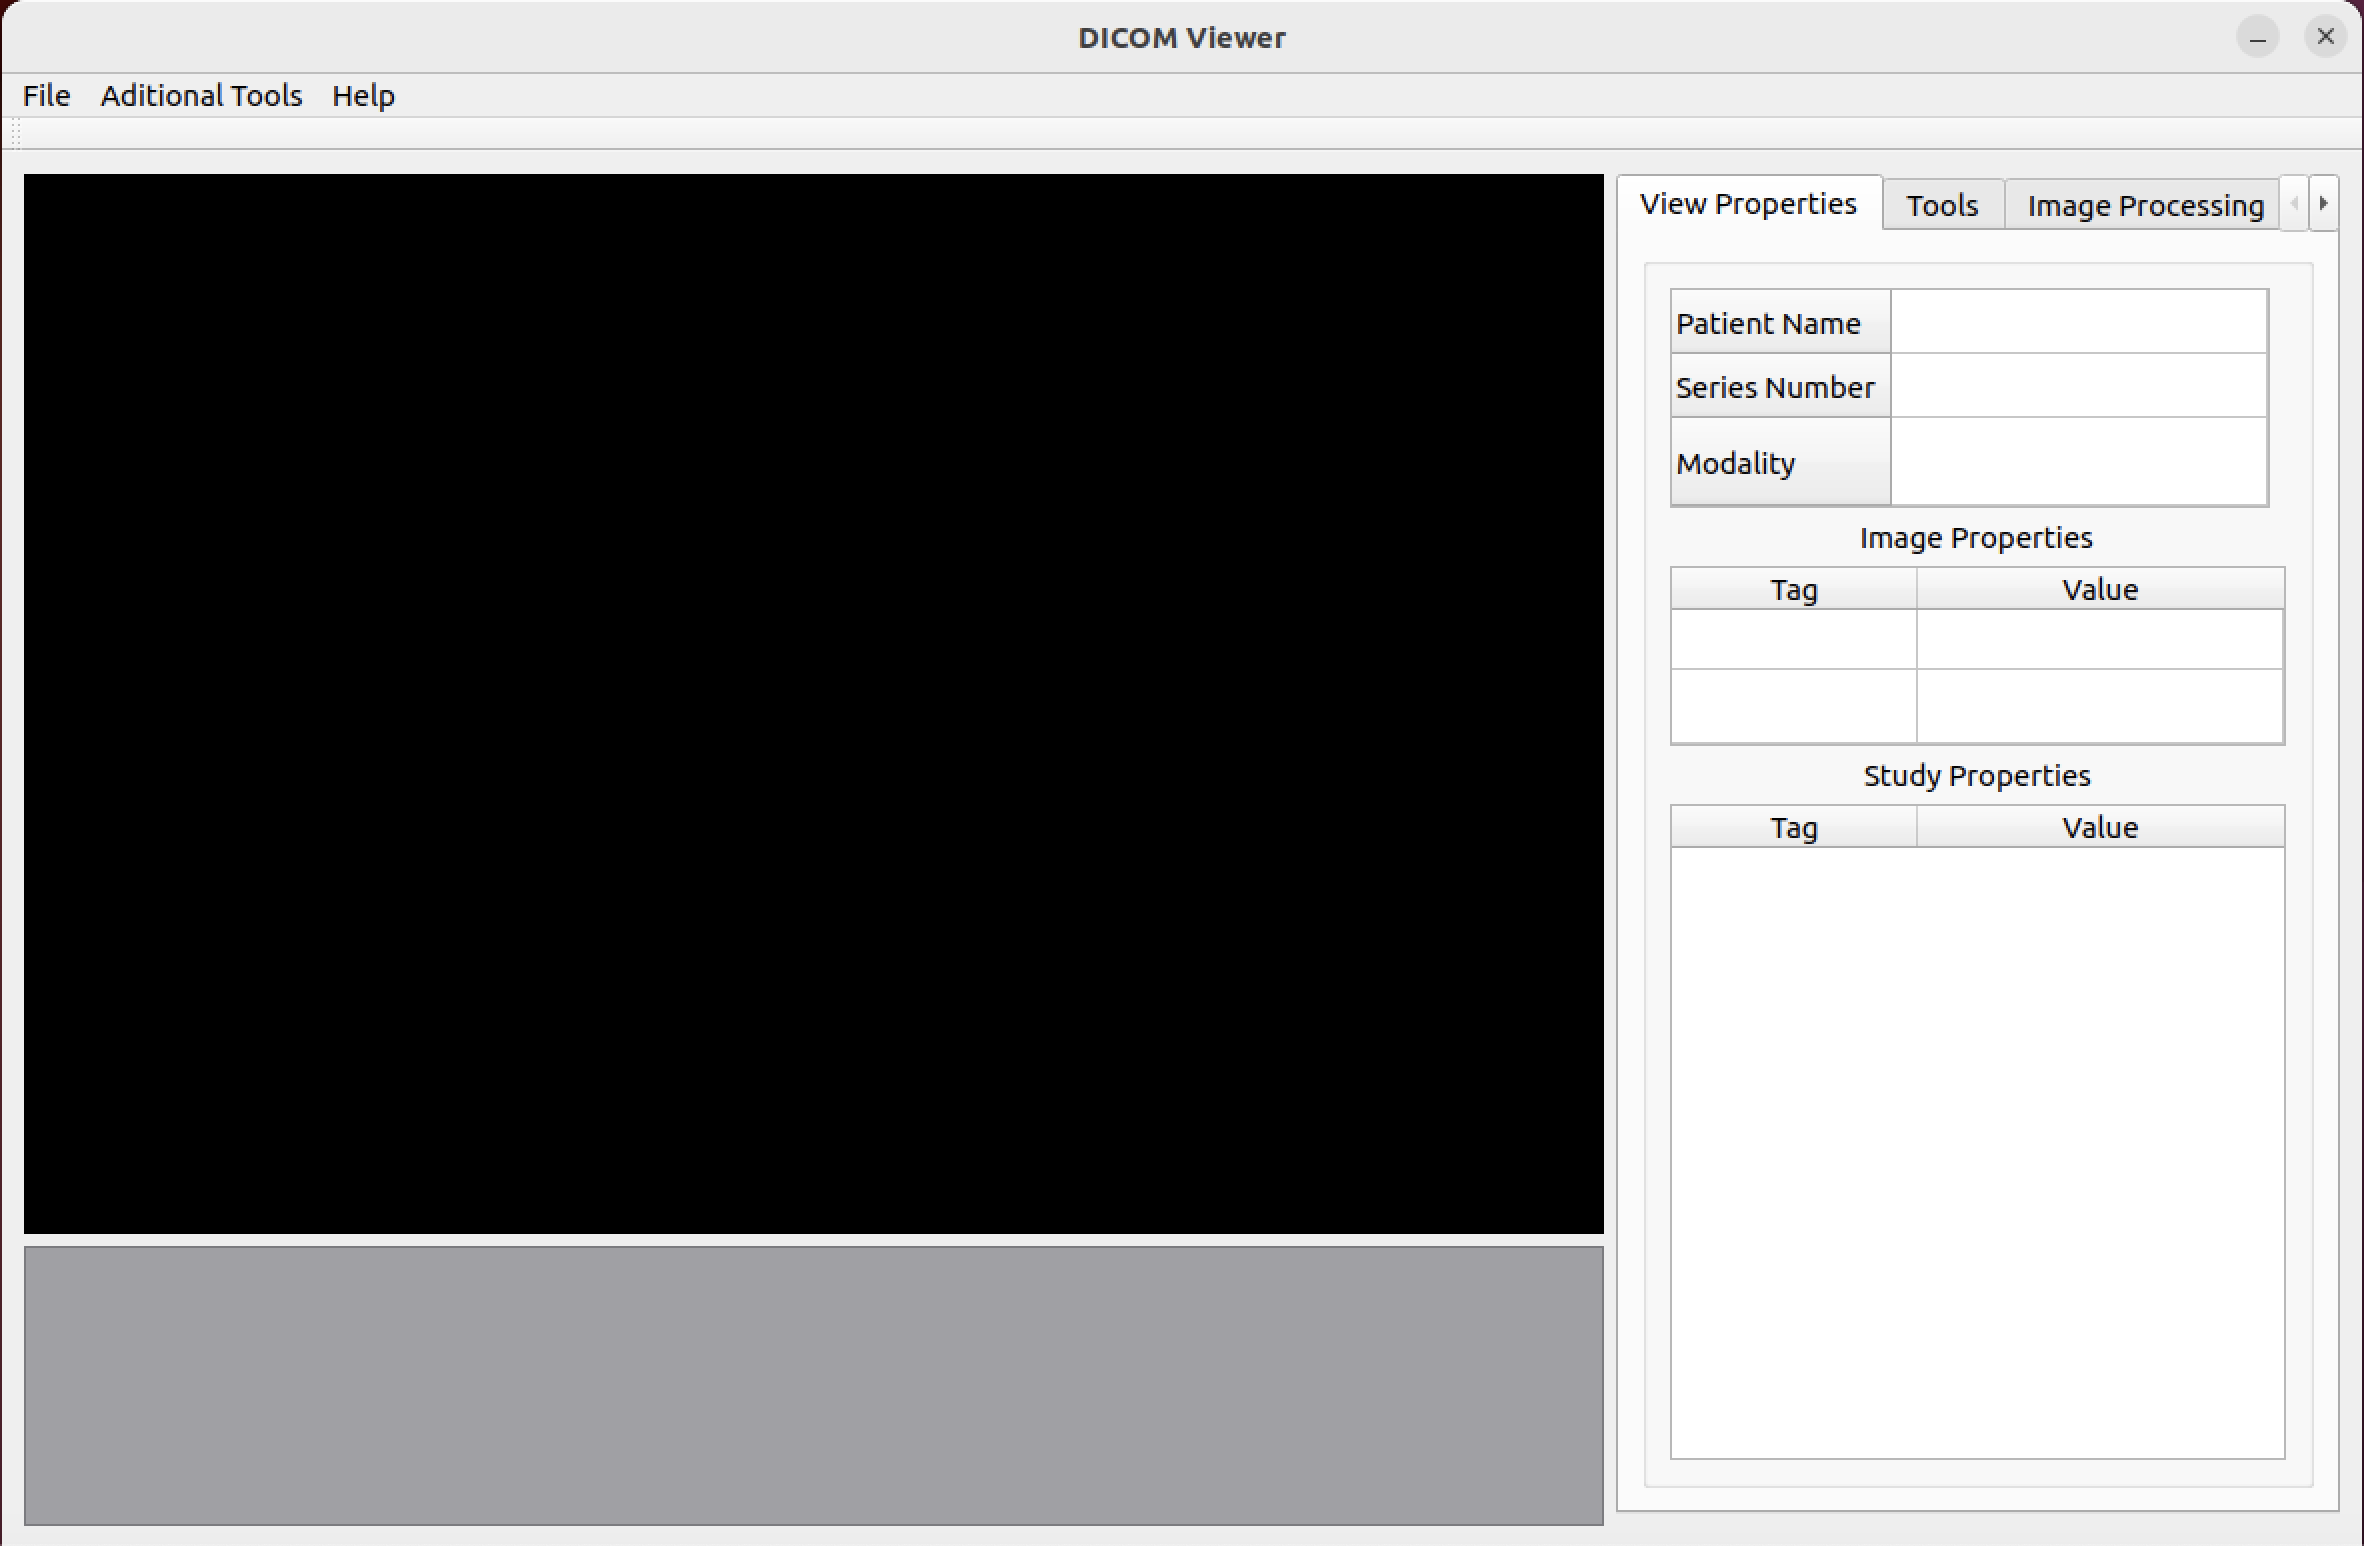
\includegraphics[height=8cm]{media/existing_app/init.png}
        \captionof{figure}[Ukážka DICOM Viewer aplikácie po spustení]{Ukážka DICOM Viewer aplikácie po spustení}
\end {center}

To sa docieli pomocou zvolenia možnosti File \rightarrow{ Open} z aplikačného menu. Následne sa otvorí systémové okno pre výber priečinka s DICOM snímkami, ktoré sa majú zobraziť v aplikácii. Bohužiaľ, nie je možné zvoliť snímky jednotlivo z priečinku, čo zapríčiní načítanie všetkých snímok z daného priečinku do aplikácie. Po zvolení priečinku sa zobrazí prvý snímok v aplikácii. Po výbere ľubovolnej možnosti, ktoré ponúka Aditional [sic] Tools menu, sa taktiež zobrazí ľavý postranný panel v aplikácii, ako je možné vidieť na snímke aplikácie nižšie. V tomto prípade bola zvolená možnosť \uv{Grid Tools}, nakoľko sa analýza súčasnej aplikácie zameriava najmä na vykreslenie mriežky a nastavenie jej parametrov, ktoré sa zobrazia práve po zvolení tejto možnosti.

\begin {center}
        \centering
        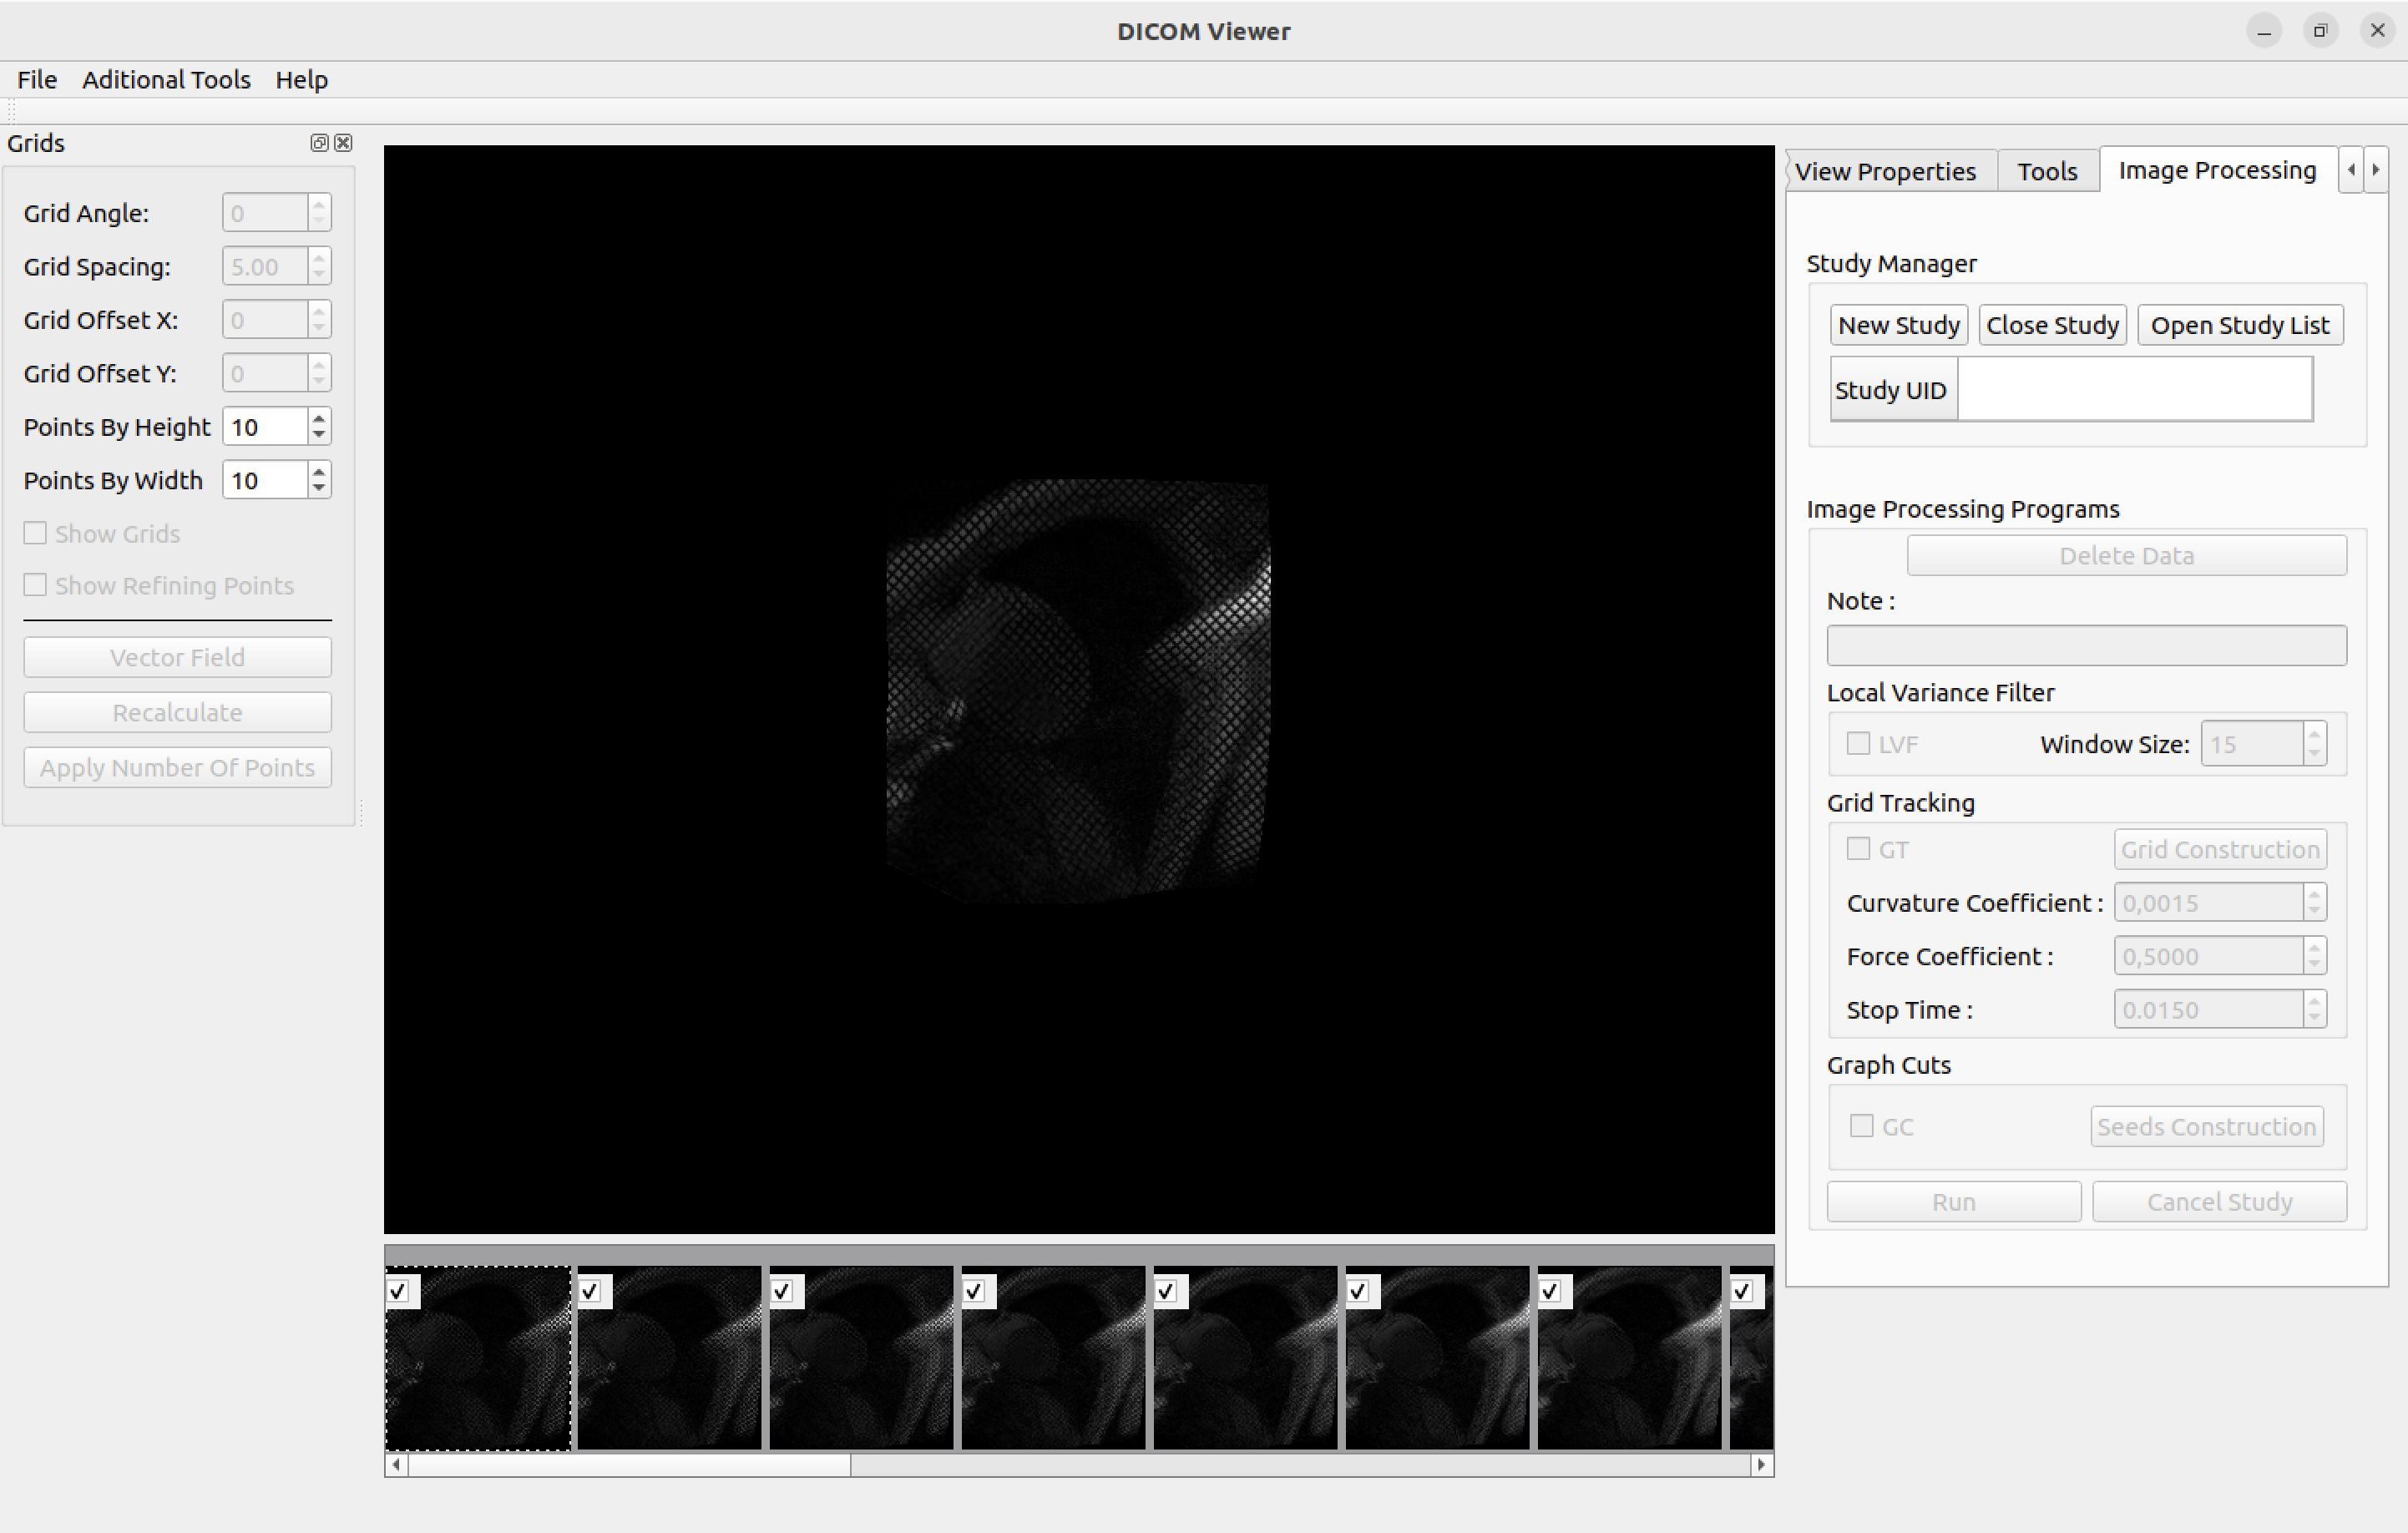
\includegraphics[height=8cm]{media/existing_app/app_with_grids_panel.png}
        \captionof{figure}[Zobrazenie prvej snímky v DICOM Viewer aplikácii]{Zobrazenie prvej snímky v DICOM Viewer aplikácii}
\end {center}

Po zobrazení ľavého postranného panelu sa odhalí celková štruktúra používateľského rozhrania aplikácie.
Tú môžeme rozdeliť na ľavý a pravý postranný panel, medzi ktorými sa nachádza čierna plocha zobrazujúca vybranú snímku. Pod touto snímkou sú zobrazené náhľady všetkých snímok. \newline

Obsahom čiernej plochy, ktorá je dominantná v zobrazení aplikácie, je aktuálne vybraná DICOM snímka. Nad ňou môže byť tiež vykreslená používateľom definovaná mriežka. Náhľady všetkých snímkov, ktoré sa zobrazujú pod aktuálne vybranou snímkou, obsahujú taktiež zaškrtávacie políčko. Toto políčko reprezentuje možnosť, či má byť daný snímok spracovaný v rámci daných 3 podprogramoch.

Obsah pravého postranného panelu je rozdelený na nasledovné karty: \uv{View Properties}, \uv{Tools}, \uv{Image Processing} a \uv{History}.

\begin {center}
        \centering
        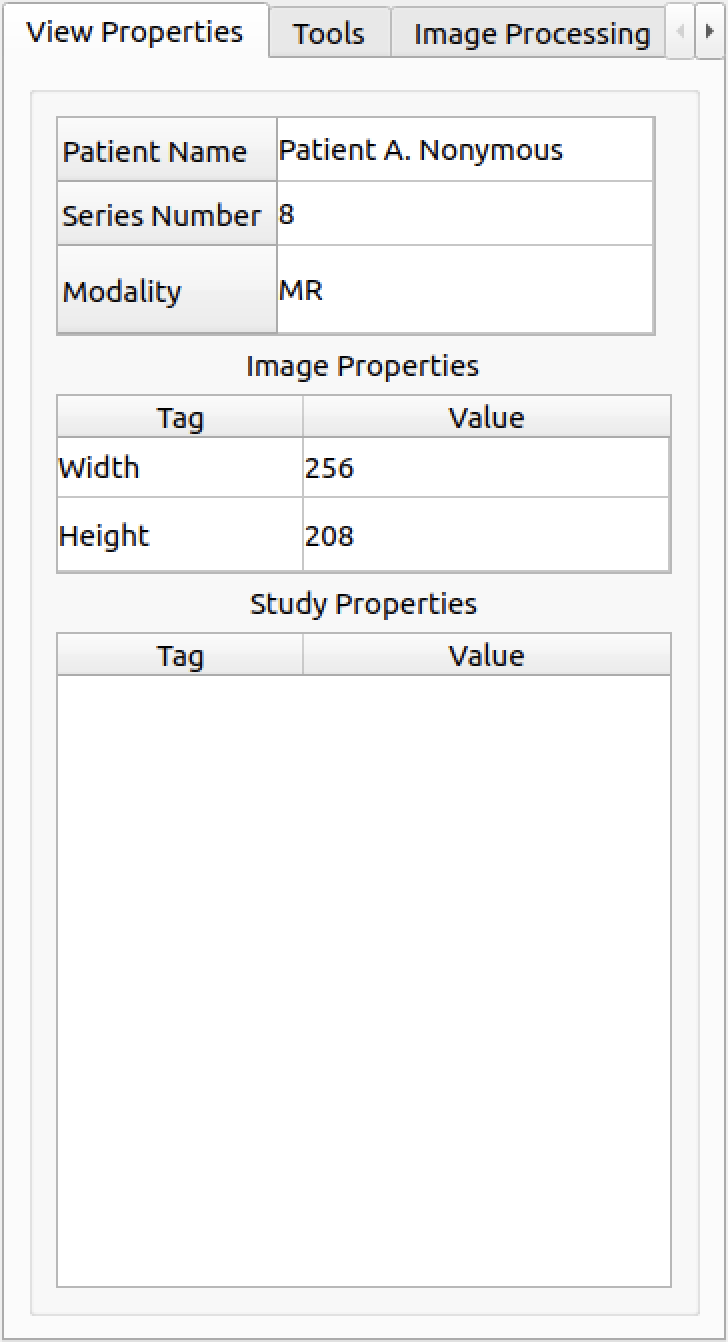
\includegraphics[width=3.5cm, height=6.10cm]{media/existing_app/tabs/view_properties.png}
        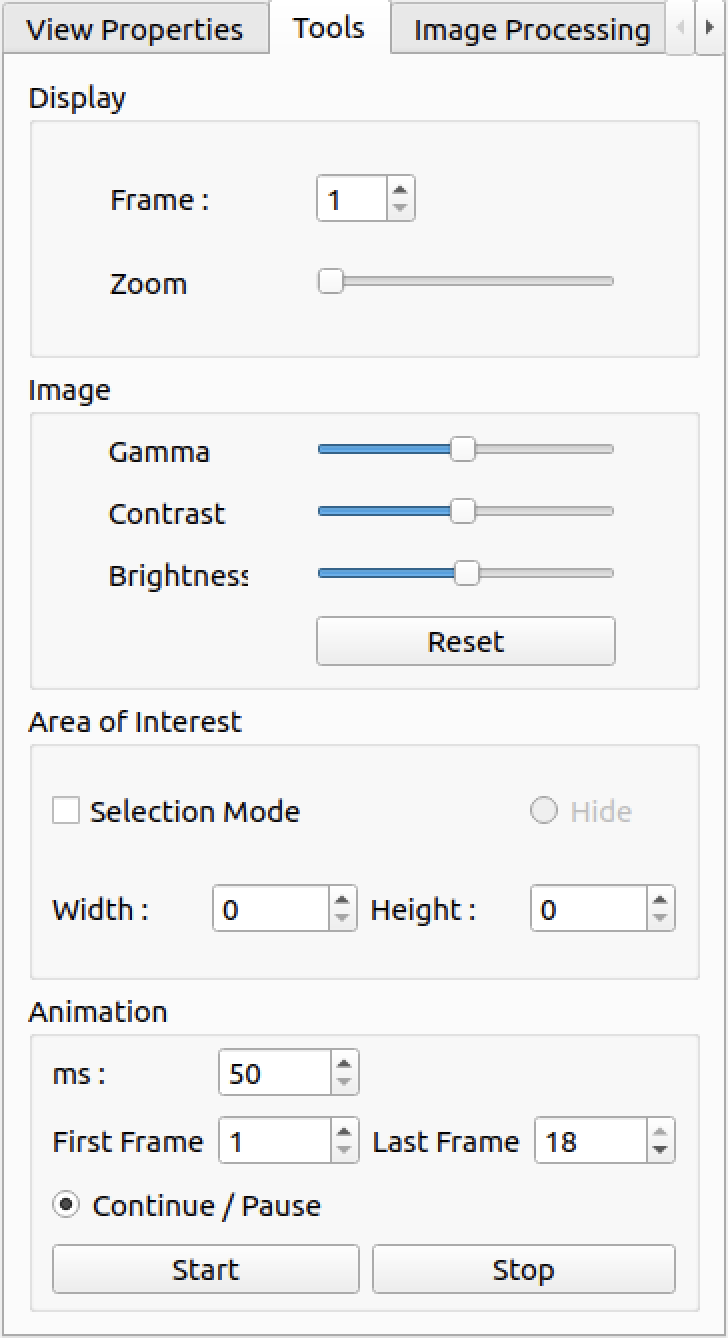
\includegraphics[width=3.5cm, height=6.10cm]{media/existing_app/tabs/tools.png}
        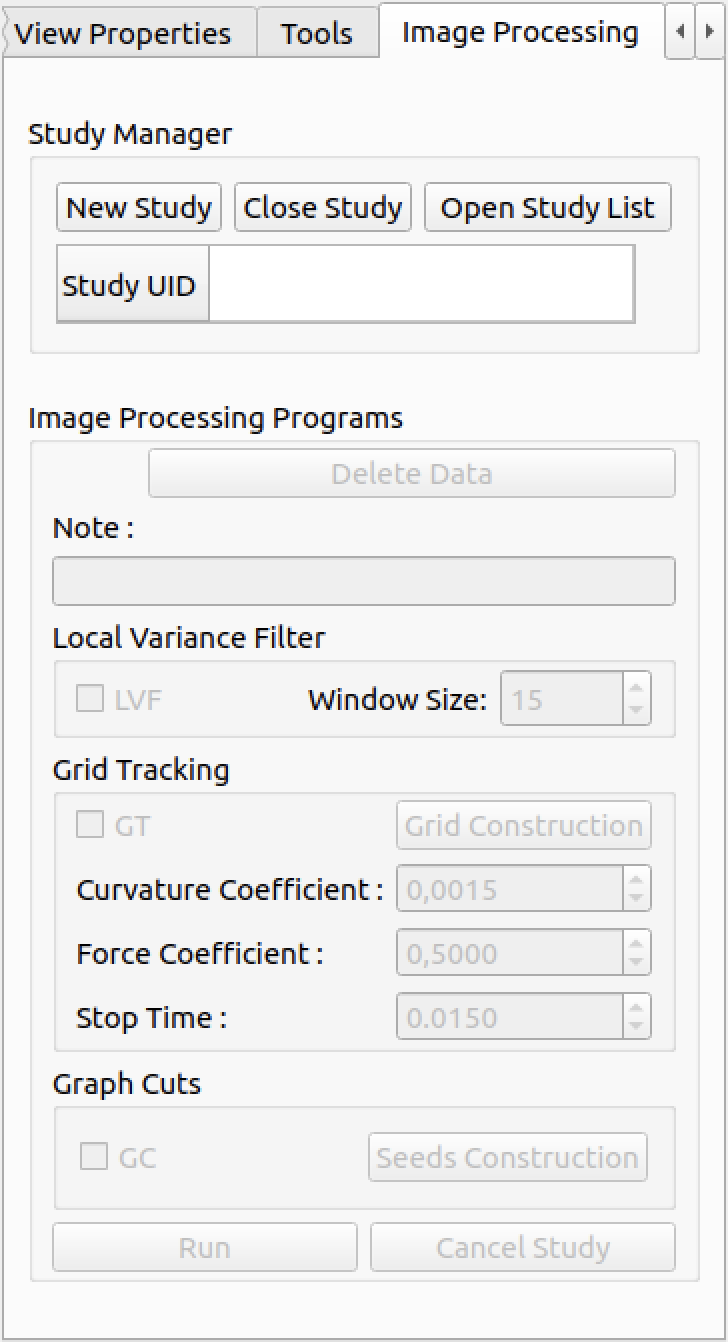
\includegraphics[width=3.5cm, height=6.10cm]{media/existing_app/tabs/image_processing_inactive.png}
        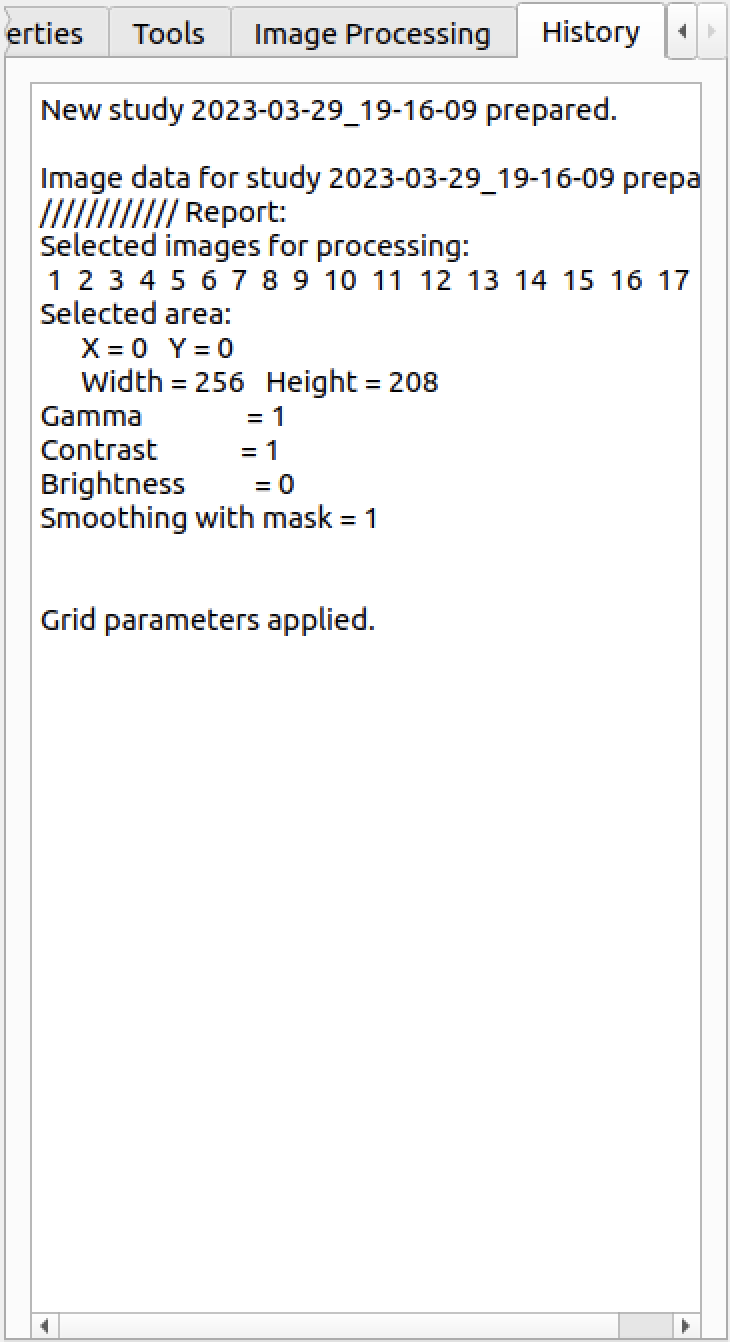
\includegraphics[width=3.5cm, height=6.10cm]{media/existing_app/tabs/history.png}
        \captionof{figure}{Zobrazenie obsahu kariet na pravom postrannom paneli}
\end {center}

\uv{View Properties} karta nie je interaktívna -- zobrazuje informácie ako meno subjektu so zobrazenou snímkou, číslo série a modalitu snímkov. Taktiež je zobrazená výška a šírka aktuálne zobrazeného snímku.

Narozdiel od predchádzajúcej karty, \uv{Tools} karta obsahuje interaktívne prvky, ako napr. zobrazenie a zmena indexu zobrazeného snímku, či slider pre priblíženie snímku. Samotnému snímku je možné tiež zmeniť kontrast, jas a gammu pomocou sliderov. Nasleduje sekcia pre nastavenie  oblasti záujmu, pri ktorej je možné nastaviť jej zobrazenie alebo zmeniť jej výšku/šírku -- oblasť záujmu je na základe týchto nastavení vykreslená nad snímkou. Keďže aplikácia podporuje prehrávanie snímkov ako animáciu, aplikácia ponúka nastavenie jej rýchlosti v milisekundách (čo predstavuje čas, ktorý ubehne zobrazením jednej snímky), nastavenie počiatočnej snímky, od ktorej sa animácia spustí, a poslednej snímky, po ktorú animácia bude spustená. Okrem nastavenia parametrov animácie nesmú chýbať tlačidlá pre samotné spustenie a zastavenie animácie.

Na ďalšej karte \uv{Image Processing} sa nachádzajú tlačidlá ovládajúce manažéra štúdií. Tento \uv{manažér} zoskupuje rôzne štúdie, pod ktorými sa ukladajú rôzne parametre aplikácie. Po kliknutí na tlačidlo \uv{Open Study List} sa zobrazí nové okno so všetkými štúdiami a ich parametrami.
Pre interakciu s ostatnými poliami na tejto karte je potrebné najprv vytvoriť novú štúdiu kliknutím na tlačidlo \uv{New Study}. Štúdiu je tiež možné ukončiť zvolením tlačidla \uv{Close Study}. Každá štúdia je reprezentovaná jedinečným ID, ktoré sa skladá z dátumu a času jej vytvorenia.
Vytvorením novej štúdie sa aktivujú polia \uv{Image Processing Programs} sekcie. Táto sekcia ponúka tri hlavné začiarkavacie políčka -- prvé reprezentuje spustenie aplikovania filtra lokálnej variancie. Druhé z nich reprezentuje spustenie algoritmu pre zarovnanie vygenerovanej mriežky s mriežkou myokardu vytvorenou pomocou SPAMM techniky a tretie spustenie algoritmu segmentácie srdečných komôr pomocou grafových rezov. Zaškrtnutím daného políčka a kliknutím na tlačidlo \uv{Run} sa algoritmus príslušný danému políčku spustí. Pre \uv{Grid Tracking} algoritmus je v tejto sekcii možné definovať tri parametre, a to \uv{Curvature Coefficient}, \uv{Force Coefficient} a \uv{Stop Time} (viď \ref{helper_apps}).

Účelom poslednej karty \uv{History} je výpis rozličných záznamov pre informovanie používateľa o prebiehajúcich krokoch aplikácie. \newline

Obsah ľavého postranného panelu sa mení v závislosti na zvolenej možnosti z menu Aditional [sic] Tools. Momentálne sa zobrazuje obsah ľavého panelu po zvolení možnosti \uv{Grid Tools}. V paneli je možné nájsť nasledujúce nastavenia:

\begin {itemize}
\item {Grid Angle -- nastavuje uhol mriežky,}
\item {Grid Spacing -- nastavuje rozpätie jednotlivých bodov,}
\item {Grid Offset X -- $x$ pozícia od ľavého horného bodu,}
\item {Grid Offset Y -- invertovaná $y$ pozícia od ľavého horného bodu,}
\item {Points by Height -- udáva počet bodov na úsečku mriežky na výšku,}
\item {Points By Width -- udáva počet bodov na úsečku na šírku,}
\item {Show Grids -- indikuje, či má byť zobrazená mriežka,}
\item {Show Refining Points -- indikuje, či majú byť zobrazené body, ktoré upresňujú pozíciu mriežky,}
\item {Vector Field -- spočíta rozdiel v pohybe mriežky medzi predchádzajúcou a aktuálnou snímkou,}
\item {Recalculate -- odošle dáta \texttt{grid-tracker} podprogramu pre opätovné zarovnanie mriežky voči SPAMM mriežke,}
\item {a Apply Number of Points -- uloží mriežku ako textový TNL multivektor}
\end {itemize}

Ostatné dve možnosti z menu \uv{Aditional [sic] Tools} nie je potrebné pre účely tejto práce popisovať.

%Pre analýzu srdcového svalu je potrebné najprv do aplikácie nahrať sériu snímkov, ktoré sú otagované priestorovou moduláciou magnetizácie popísanou vyššie. Táto mriežka sa na každom snímku deformuje podľa pohybu tkaniva. Na počiatočných snímkoch je mriežka dobre viditeľná, avšak jej viditeľnosť sa každým ďalším snímkom zmenšuje. Tento efekt je spôsobený poklesom Nevýhodou  Pohyb myokardu je možný analyzovať vďaka 


\section {Analýza požiadaviek}
\todo {Presunúť do návrhu po rozhodnutí o architektúre aplikácie?}
Táto sekcia sa venuje analýze požiadaviek, ktoré sa delia na dve hlavné kategórie. Týmito kategóriami sú funkčné a nefunkčné požiadavky.
Na základe týchto požiadaviek bude možné implementovať novú aplikáciu pre potreby analýzy srdcového myokardu.

\subsection {Funkčné požiadavky}
Funkčné požiadavky sú požiadavky vymedzujúce rozsah funkcionality, ktorá by mala byť v danej aplikácii implementovaná.

\subsubsection {Spracovanie a zobrazenie MR snímkov}\label{mr_images_processing}
Do aplikácie by malo byť možné importovať snímky z magnetickej rezonancie vo formáte DICOM a tieto snímky taktiež zobraziť.

\subsubsection {Animácia MR snímkov}\label{animation}
Aplikácia by mala umožniť animovať importované snímky pre jednoduchšiu analýzu pohybu myokardu. Parametre animácie ako jej rýchlosť a výber fotky, od/do ktorej snímky má animácia prebiehať by mali byť upraviteľné, napr. pomocou číselného vstupu.

\subsubsection {Zobrazenie a interaktívna úprava mriežky}\label{grid_show}
Implementovaná aplikácia by mala vedieť zobraziť mriežku nad snímkou z MR, ktorá by sa mala dať vygenerovať tlačidlom v používateľskom rozhraní. Mriežka by taktiež mala byť interaktívna, t.j. polohu jej bodov by bolo možné interaktívne upravovať, najlepšie pomocou potiahnutím bodu myšou. Parametre tejto mriežky (\ref{old_ui}) by sa taktiež mali dať upraviť podľa želania používateľa a ich zmena by mala byť ihneď viditeľná.

\subsubsection {Zadanie parametrov pre \texttt{grid-tracker} podprogram}\label{grid_paremeters}
Pre korektné spustenie \texttt{grid-tracker} podprogramu pre zarovnanie mriežky je nutné tomuto podprogramu podsunúť rozličné parametre. Tieto parametre by sa mali dať definovať v aplikácií pre ich neskoršie použitie v tomto podprograme. Výpis týchto parametrov je možné nájsť v \ref{helper_apps}.

\subsubsection {Spustenie \texttt{grid-tracker} podprogramu a zobrazenie jeho výsledkov}\label{grid_results}
Aplikácia by mala umožniť spustiť \texttt{grid-tracker} podprogram, ktorý zarovná mriežku definovanú používateľom s mriežkou, ktorá bola vygenerovaná pomocou techniky SPAMM. Po jej zarovnaní by mala byť aplikácia schopná vykresliť upravenú mriežku.

\subsection {Nefunkčné požiadavky}
Požiadavky tohto typu síce nevymedzujú rozsah funkcionality danej aplikácie, avšak umožňujú určiť isté obmedzenia pre novú aplikáciu, ako napr. dôraz na podobu výslednej architektúry aplikácie.

\subsubsection {Webová aplikácia}

Prvou nefunkčnou požiadavkou je vytvorenie webovej aplikácie, ktorá by mala byť prístupná zo všetkých moderných webových prehliadačov. Pre lekárov výber tejto architektúry zjednoduší jej prístupnosť, nakoľko k takejto aplikácii bude možné pristupovať z rôznych zariadení a platforiem bez nutnosti inštalácie aplikácie a jej následnej podpory na týchto zariadeniach.

\subsubsection {Používateľské rozhranie}

Pre interakciu s aplikáciou je nutné navrhnúť a implementovať používateľské rozhranie, pomocou ktorého lekári budú môcť s aplikáciou interagovať. Lekári by preferovali používateľské rozhranie podobné iným aplikáciám z tejto oblasti.

\subsubsection {Ochrana pred únikom dát o pacientovi}

Práca s osobnými dátami by mala byť do maximálnej možnej miere naprieč aplikáciou minimalizovaná, aby sa predišlo únikom citlivých údajov o pacientovi. Týka sa to najmä práce s DICOM súbormi, nakoľko tie obsahujú citlivé dáta o pacientovi.

\section {Používateľské role}

V aplikácii sa bude nachádzať len jeden typ používateľa rovnako ako v súčasnej aplikácii. Tomuto používateľovi by mala teda byť aplikácia sprístupnená bez rôznych funkčných obmedzení.

\section {Prípady použitia}
Nasledujúce prípady použitia reprezentujú rôzne činnosti, ktoré môže používateľ s aplikáciou vykonávať. Tieto prípady použitia sú popísané pomocou scenárov, ktoré taktiež vychádzajú z funkčných požiadaviek kladených na novú aplikáciu.

\subsection {UC1 -- Zobrazenie snímkov v aplikácii}\label{uc1}
Zobrazenie snímkov magnetickej rezonancie v DICOM formáte je jedným z esenciálnych funkčných požiadaviek -- \uv{\nameref{mr_images_processing}}. Nasledovný scenár túto požiadavku realizuje.

\subsubsection*{Scenár:}
\begin {enumerate}
\item {Používateľ klikne na jedno z tlačidiel pre import DICOM snímkov do aplikácie.}
\item {Prehliadač zobrazí systémové okno, v ktorom si používateľ vyberie snímky, ktoré by chcel mať zobrazené v aplikácii.}
\item {Následne potvrdí import želaných snímkov kliknutím na tlačidlo \uv{Otvoriť}.}
\item {Aplikácia automaticky vykreslí prvý importovaný snímok a taktiež zobrazí náhľady ostatných importovaných snímkov.}
\item {V prípade, že sa medzi zvolenými snímkami nachádza súbor, ktorý nekorešponduje so štruktúrou DICOM súboru, aplikácia zobrazí notifikáciu o neúspešnom zobrazení snímky.}
\end {enumerate}
	
\subsection {UC2 -- Animácia snímkov}
Nasledovný scenár realizuje funkciu prehrania série snímkov ako animáciu, ako bolo popísané vo funkčnej požiadavke \uv{\nameref{animation}}.
Okrem iného taktiež zahŕňa prípad \uv{\nameref{uc1}}. 

\subsubsection*{Scenár:}
\begin {enumerate}
\item {\nameref{uc1}.}
\item {Kliknutím na tlačidlo reprezentujúce štart animácie sa spustí animácia importovaných snímkov.}
\item {Kliknutím na tlačidlo reprezentujúce koniec animácie sa animácia skončí.}
\end {enumerate}

\subsubsection*{Alternatívny scenár:}
\begin {enumerate}
\item [\textbf{2.}] {Používateľ si nastaví rýchlosť animácie, index snímku, od ktorého má animácia začínať alebo index snímku, ktorým má animácia končiť.}
\item  [\textbf{3.}] {Kliknutím na tlačidlo reprezentujúce štart animácie sa spustí animácia importovaných snímkov.}
\item  [\textbf{4.}] {Kliknutím na tlačidlo reprezentujúce koniec animácie sa animácia skončí.}
\end {enumerate}

\subsection {UC3 -- Vytvorenie mriežky}\label{uc3}
Vytvorenie mriežky nad snímkou z MR je potrebné pre účely analýzu pohybu myokardu. Nasledujúci scenár čiastočne realizuje túto funkčnú požiadavku definovanú v \ref{grid_show}. Taktiež zahŕňa prípad použitia \uv{\nameref{uc1}}.

\subsubsection*{Scenár:}
\begin {enumerate}
\item {\nameref{uc1}.}
\item {Používateľ klikne na tlačidlo \uv{Create grid}.}
\item {Aplikácia zobrazí výzvu pre kliknutie na oblasť snímky, kde má byť mriežka vytvorená.}
\item {Používateľ klikne na oblasť snímky, kde chce vytvoriť mriežku.}
\item {Aplikácia vygeneruje mriežku s predvolenými nastaveniami a zobrazí ju.}
\end {enumerate}

\subsection {UC4 -- Úprava parametrov mriežky}\label{uc4}
Medzi prípady použitia patrí aj úprava parametrov mriežky určenej pre analýzu pohybu srdcového svalu. Nakoľko je najprv potrebné mať mriežku  pred jej úpravou vytvorenú, zahŕňa nasledovný scenár aj jej vytvorenie. Ten taktiež čiastočne realizuje funkčnú požiadavku \uv{\nameref{grid_show}}.

\subsubsection*{Scenár:}
\begin {enumerate}
\item {\nameref{uc3}.}
\item {Používateľ upraví jeden alebo viacero parametrov uvedených v \ref{old_ui}.}
\item {Aplikácia následne automaticky vykreslí mriežku na základe upravených parametrov.}
\end {enumerate}

\subsection {UC5 -- Zadanie parametrov pre \texttt{grid-tracker} podprogram}\label{uc5}
Pre spustenie algoritmu zodpovedného pre posun mriežky vytvorenej používateľom voči mriežke vygenerovanej SPAMM technikou je potrebné tomuto algoritmu poslať tri parametre definované v \ref{old_ui}. Nasledujúci scenár tento prípad použitia realizuje spolu s funkčnou požiadavkou -- \uv{\nameref{grid_parameters}}.

\subsubsection*{Scenár:}
\begin {enumerate}
\item {\nameref{uc1}.}
\item {Používateľ zadá číselné hodnoty parametrov \uv{Curvature coefficient}, \uv{Force coefficient} a \uv{Stop time}.}
\end {enumerate}

\subsection {UC6 -- Spustenie podprogramu a zobrazenie výsledku}
Spustenie samotného algoritmu vyžaduje mať importované DICOM snímky v aplikácii, vytvorenú mriežku s upravenámi parametrami a zadaním parametrov pre \texttt{grid-tracker} podprogram. To je dôvodom, prečo tento scenár použitia zahŕňa prípady \uv{\nameref{uc1}}, \uv{\nameref{uc3}}, \uv{\nameref{uc4}} a \uv{\nameref{uc5}}. Samotný scenár realizuje funkčnú požiadavku \uv{\nameref{grid_results}}.

\subsubsection*{Scenár:}
\begin {enumerate}
\item {\nameref{uc1}}.
\item {\nameref{uc3}}.
\item {\nameref{uc4}}.
\item {\nameref{uc5}}.
\item {Používateľ kliknutím na tlačidlo \uv{Compute} spustí výpočet pomocou \texttt{grid-tracker} podprogramu.}
\item {Po dokončení výpočtu aplikácia zobrazí mriežky upravené horeuvedeným podprogramom.}
\end {enumerate}


\section {Analýza frameworkov pre tvorbu webového rozhrania}

\section {Analýza spracovania MR snímkov vo webovej aplikácii}

\section {Analýza možnostu prepojenia webového rozhrania s \texttt{grid-tracker} podprogramom}